\chapter{paired t-test}

The used method of the study design is called in series design. This enable to compare the situation before and after treatment within each subject.
\begin{figure}[H]
	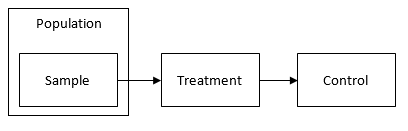
\includegraphics[width=0.4\textwidth]{figures/inseries1}
	\caption{The procedure of studies with in series design.}
	\label{fig:FigureLABEL}
\end{figure}

Within this study the arms of the subjects will be cuffed. To avoid any carry-over effect, the measurements on the normal arm will be done first. That means beginning with the control and then the "treatment".
\begin{figure}[H]
	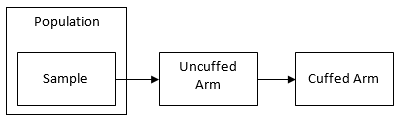
\includegraphics[width=0.4\textwidth]{figures/inseries2}
	\caption{The procedure of this study with in series design.}
	\label{fig:FigureLABEL}
\end{figure}

The paired t-test is used to check the difference of means of two conditional samples. This test is usually used to compare "before treatment" and "after treatment".
It is requisite that the sample size of the of both samples is identical.
Following some useful formulas:
\begin{itemize}
	\item test variable
	\begin{flalign}
		t=\frac{\bar{X_{D}}-\mu_{0}}{\frac{s_{D}}{\sqrt{n}}}
	\end{flalign}
	\item mean of difference of the paired means
	\begin{flalign}
		\bar{X_{D}}=\frac{1}{n}\times \Sigma (X_{1}-X_{2})
	\end{flalign}
	\item standard derivation of the difference of the paired means
	\begin{flalign}
		s_{D}=\sqrt{\frac{\Sigma((X_{1}-X_{2})-\bar{X_{D}})^{2}}{n-1}}
	\end{flalign}
	\item degree of freedom
	\begin{flalign}
		2\times n-2
	\end{flalign}
\end{itemize}